\documentclass[10pt,letterpaper]{article}

\usepackage{hyperref}
\usepackage{cogsci}
\usepackage{pslatex}
\usepackage{pdfsync}
\usepackage{apacite}
\usepackage{amsmath}
\usepackage{graphicx}
\usepackage{topcapt}
\usepackage{color}
\usepackage[textsize=small,textwidth=1.8cm]{todonotes}

\setlength{\marginparwidth}{1.5cm}

\title{The pragmatics of negation across contexts}

\author{{\large \bf Ann E. Nordmeyer} \\ \texttt{anordmey@stanford.edu}\\ Department of Psychology \\ Stanford University \\ 
\And {\large \bf Michael C. Frank} \\ \texttt{mcfrank@stanford.edu} \\ Department of Psychology \\ Stanford University \\ }

\begin{document}

\maketitle


\begin{abstract}
Why do some negative sentences sound strange, even when they are both true and grammatical? We explore the pragmatics of negation by examining adults' explicit felicity judgments of negative sentences in context.  In Experiment 1, we found that a pragmatically supportive context elicited higher felicity ratings for negative sentences, and that negative sentences expressing nonexistence were rated higher than negative sentences referring to an alternative object.  In Experiment 2, we used a within-subjects design to compare three context types, and found that negative sentences were rated more felicitous in a context where most of the characters possessed the negated object, compared to contexts where the other characters possessed an alternative object or nothing.  We discuss the pragmatics of negation in light of these results, arguing that the felicity of negative sentences is influenced by changes in the informativeness of these sentences in different contexts. 

\textbf{Keywords:} 
Negation; felicity judgments; pragmatics
\end{abstract}

\section{Introduction}

A sentence that is both grammatical and true can nevertheless sound odd in some contexts. If you open a mysterious box and find that it is empty, it's weird to say ``This box doesn't have any chocolates in it,'' despite the truth of the proposition. But the same sentence becomes perfectly reasonable if you are in a chocolate store surrounded by boxes filled with chocolate.  Why do some sentences sound strange (\emph{infelicitous}) in one situation, but normal in another?

Theories of pragmatics attempt to provide an account of how language users move from the literal semantics of a sentence to an inference about the speaker's intended meaning. For example, according to Grice's \citeyear{grice1975} Cooperative Principle, speakers should produce utterances that are truthful, relevant, and informative.  By assuming that speakers do so, listeners can make inferences about intended meaning that go beyond the sentence's literal meaning. Modern neo-Gricean theories tend to derive such inferences from the tension between being informative with respect to a communicative goal and minimizing the effort expended \cite{horn1984,levinson2000,frank2012}. These theories make predictions about sentence felicity: As in our example above, a sentence that is not pragmatically optimal can sound strange even when it is both grammatical and true.

We explore this relationship between contextual pragmatics and felicity using negation. As the previous example demonstrates, negative sentences are particularly sensitive to the effects of context, making them a good case study.  When they are presented without any context, negative sentences are difficult to process relative to positive sentences \cite{hclark1972, carpenter1975, just1971, just1976}, but supportive contexts can substantially reduce this processing difficulty \cite{wason1965, glenberg1999, ludtke2006, nieuwland2008, dale2011, nordmeyer2014}.   Previous work has linked reaction time to syntactic surprisal, an information-theoretic measure predicting that low-probability utterances will be processed slower than high-probability utterances \cite{levy2008}.  If \emph{pragmatic surprisal}---the probability of an utterance being produced given the context---is responsible for the context effects seen in negation processing, these context effects should be reflected in adults' explicit felicity judgments as well.   

We focus on two types of negation: \emph{nonexistence} and \emph{alternative} negation.  The same sentence can express either of these concepts depending on the context.  For example, the sentence ``This box doesn't contain chocolate'' might refer to an empty box (e.g. nonexistence) or a box containing some alternative object (e.g. broccoli instead of chocolate).  Previous work suggests that adults are faster to identify the referent of nonexistence negation compared with alternative negation \cite{nordmeyer2013, nordmeyer2014b}, but it is not clear if this difference is due to processing demands (e.g. identifying a missing feature is superficially easier than identifying a changed feature), or if it reflects an expectation about the pragmatics of negation.  Adults may find alternative negation infelicitous because they expect the sentence to describe present, rather than absent, features.

We examined the effects of a pragmatic context on adults' explicit felicity judgments for different negative sentences.  In Experiment 1, we tested the effect of context on nonexistence negation and alternative negation.  We found that negative sentences presented in a supportive context were rated as more felicitous, and that nonexistence negation was rated higher than alternative negation.  In Experiment 2, we found that alternative negation was rated as more felicitous in a context where all of the other characters possessed the negated object, compared to contexts where the other characters possessed the alternative object or no object.  We discuss these results within a neo-Gricean framework, demonstrating that a model of informativeness can predict the same qualitative pattern seen in our data.  Together these findings suggest that adults' felicity judgments reflect preferences for negative sentences that are more informative given the context.  

\section{Experiment 1}

Experiment 1 explored how different contexts (see Figure \ref{fig:trial}) affected participants' felicity ratings for negative sentences.  Half of the participants in Experiment 1 saw sentences presented in a context where none of the surrounding characters had any objects (the \emph{none} condition), and the other half saw sentences presented in a context where everyone except for the target character possessed the negated object (the \emph{target} condition).  In half of the true negative trials, the referent of the negative sentence was a character who had nothing (nonexistence negation).  In the other half of true negative trials, the referent of the sentence was a character who had some other object (alternative negation).  Finally, we examined how different syntactic framings might influence sentence judgments (``has no X'' and ``doesn't have X''). If previously seen context effects are driven by the informativeness of negation in different contexts, then these same effects should appear regardless of the syntactic framing of the sentences.  

\subsection{Method}

\subsubsection{Participants}

We recruited 94 adults (50 male, 41 female, three declined to report gender) to participate in an online experiment through Amazon Mechanical Turk.  Participants ranged in age from 18-65.  We restricted participation to individuals in the United States. We paid 35 cents for the experiment, which took approximately five minutes to complete.  

\subsubsection{Stimuli}

We created 16 trial items. On each trial, four Sesame Street characters were shown standing behind tables.  One character was randomly selected as the ``target'' character, designated by a red box (see Figure \ref{fig:trial}). The remaining three characters were designated as ``context'' characters.


\begin{figure}[t]
\begin{center} 
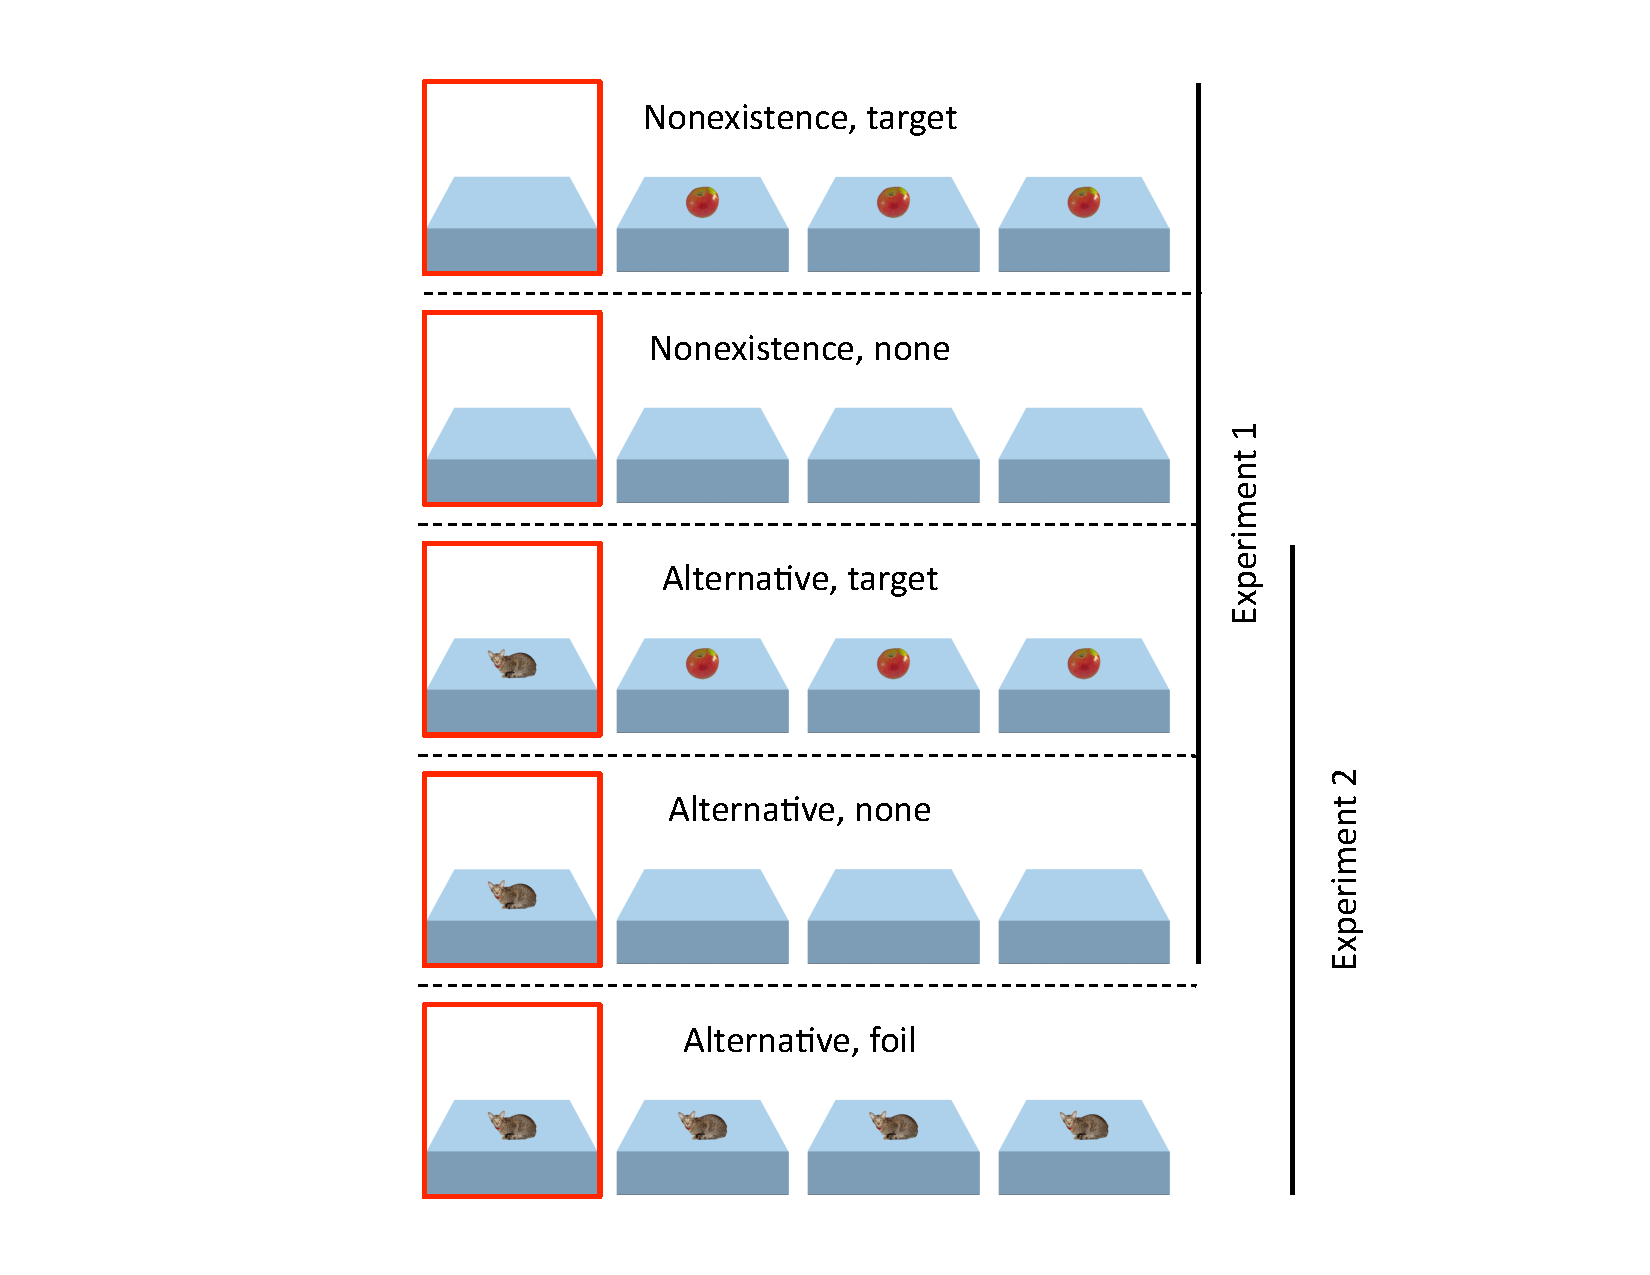
\includegraphics[width=3in]{figures/trialtypes.pdf}
\caption{\label{fig:trial} The five types of true negative trials across Experiment 1 and Experiment 2.  In this example, the target item is an apple and the alternative item is a cat. Below each set of pictures a sentence appeared about the character in red, e.g. ``Abby doesn't have an apple.''}  
\end{center} 
\end{figure}

Participants were randomly assigned to the \emph{none} context condition or the \emph{target} context condition.  In the \emph{none} condition, the context characters all stood behind empty tables.  In the \emph{target} condition, each context character had an identical object on their table.  The objects belonged to one of four categories: animals (cat, dog, horse cow), vehicles (car, bus, boat, truck), food (apple, banana, cookie, orange), and household objects (fork, spoon, bowl, plate).  Stimuli were created using images from the Bank of Standardized Stimuli \cite{brodeur2010}.  

Below the characters was a sentence about the target character.  Across the entire experiment, six of these sentences were positive sentences such as ``[character] has a/an [object].''  Five were negative sentences of the form ``[character] has no [object]'' and five were negative sentences of the form ``[character] doesn't have a/an [object].'' 

The target character either had a target object on their table, or an alternative object (``alternative'' trials), or nothing (``nonexistence'' trials).  This allowed us to examine two different negative concepts (see Figure \ref{fig:trial} for depictions of these trials and the different context conditions).    These trial conditions were crossed such that each participant saw six true positive trials, two false positive trials (one alternative and one nonexistence), two false negative trials (one ``has no'' sentence type and one ``doesn't have'' sentence type), and eight true negative trials (two ``has no''/nonexistence, two ``has no''/alternative, two ``doesn't have/nonexistence'', and two ``doesn't have/alternative'').  Each of these trial types was randomly assigned to a target object, and trials were presented in a random order.  

A slider bar was positioned beneath the sentence, with a seven-point scale ranging from ``Very Bad'' to ``Very Good.''  A progress bar at the top of the screen informed participants how much of the experiment they had completed. 

\subsubsection{Procedure}

Participants first saw an instructions screen that briefly described the task and informed them that they could stop at any time.  Once participants agreed to participate, they saw an instructions screen that explained the task in more detail.  Participants were asked to rate how ``good'' each sentence was, e.g. ``if no one would ever say a particular sentence in this context, or if it is just wrong, rank that as `Very Bad,' but if something is right and sounds perfectly normal, mark it as `Very Good.''' Participants were encouraged to use the entire scale. On each trial the pictures, sentence, and slider bar appeared simultaneously, and participants had to make a selection on the scale in order to progress to the next trial.  


\subsubsection{Data Processing}

We excluded from analysis two participants who did not list English as their native language.  Thus, data from a total of 92 participants were analyzed, 47 in the \emph{none} context condition and 45 in the \emph{target} context condition.  

\subsection{Results and Discussion}

True negative sentences were rated significantly higher in a \emph{target} context compared to a \emph{none} context. For example, the sentence ``Abby has no apples'' was rated higher when all of the other characters \emph{had} apples, compared to contexts where all of the other characters had nothing. This finding supports our hypotheses and replicates patterns previously seen in studies of processing time using explicit felicity judgments.  Negative sentences expressing nonexistence were rated as more felicitous than negative sentences referring to an alternative object (see Figure \ref{fig:s1}). True positive sentences did not show any effect of context, nor did false sentences of any sentence type, likely due to a ceiling effect for true positive sentences and a floor effect for false sentences.  
 
To test the reliability of these findings, we fit a linear mixed-effects model examining the interaction between context, negation type (e.g. nonexistence or alternative), and negation framing (e.g. ``has no X'' vs. ``doesn't have X'') on felicity ratings.\footnote{ The model specification was as follows: \texttt{rating $\sim$ context~$\times$~negation type~$\times$~negation type + (negation type~$\times$~negation frame~\textbar~subject) +  (negation type~$\times$~negation frame~\textbar~item)}.  Significance was calculated using the standard normal approximation to the $t$ distribution \cite{barr2013}. Data and analysis code can be found at \href{http://github.com/anordmey/cogsci15}{http://github.com/anordmey/cogsci15}.} Because we were primarily interested in the effects of context on true negative sentences, we focused on these trials in our analyses.  The effects of context on true negative sentences reported in both experiments are significant in full models of all sentence types as well.

Examining the model, we found a main effect of context, with true negative sentences presented in a \emph{target} context eliciting significantly higher ratings than true negative sentences presented in a \emph{none} context ($\beta= 1.08$, $p< .001$).  We found main effects of negation type, with alternative negation receiving lower ratings nonexistence negation ($\beta= -.43$, $p< .05$), as well as a marginally significant effect of negation framing, with sentences of the form ``has no X'' receiving lower ratings than sentences of the form ``doesn't have X''  ($\beta= -.49$, $p= .052$).  There were no interactions between negation frame, negation type, and context.  

Participants showed a slight preference for negative sentences with the framing ``doesn't have X'' over ``has no X''.  This preference did not interact with context or negation type; participants preferred the ``doesn't have'' framing for both alternative negation and nonexistence negation, and rated both sentence frames higher when they were presented in a \emph{target} context.  This finding suggests that effects of context on the felicity of negative sentences are not due to features of a specific syntactic frame.

In previous work we found that adults were somewhat faster to look at the referent of nonexistence negation compared with alternative negation \cite{nordmeyer2014b}. In that experiment, the difference between nonexistence and alternative negation could have arisen because of superficial, stimulus-level differences (i.e. it might be easier to identify a character with nothing than one with an alternative object). Our replication of this result using explicit felicity judgments suggests that this difference could result from pragmatic factors as well. One explanation for participants' preference for nonexistence negation is that a sentence such as ``Abby doesn't have an apple'' is more informative when Abby has nothing compared to when she has an alternative object.  In a strong context (e.g. one where everyone else has apples), using negation to point out Abby's lack of apples is informative because it uniquely identifies her character in the array.  When Abby has some alternative object (e.g. a cat), however, there is a \emph{more} informative utterance that a speaker could use (e.g. ``Abby has a cat'').  The presence of a more informative utterance makes these negative sentences less felicitous, even when they appear in context.

Overall, we found that a pragmatic context increases the felicity judgments of negative sentences.  Across all types of negative sentences, participants assigned higher ratings to sentences that were presented with a \emph{target} context compared to sentences that were presented with a \emph{none} context.  This corroborates previous work in which more informative negative sentences (based on the context) were processed faster than less informative negative sentences \cite{nordmeyer2014}.  In the next section, we expand on this finding by testing the same sentences in a new context designed to test alternative possibilities for how context affects the pragmatics of negative sentences.

\begin{figure}
\begin{center} 
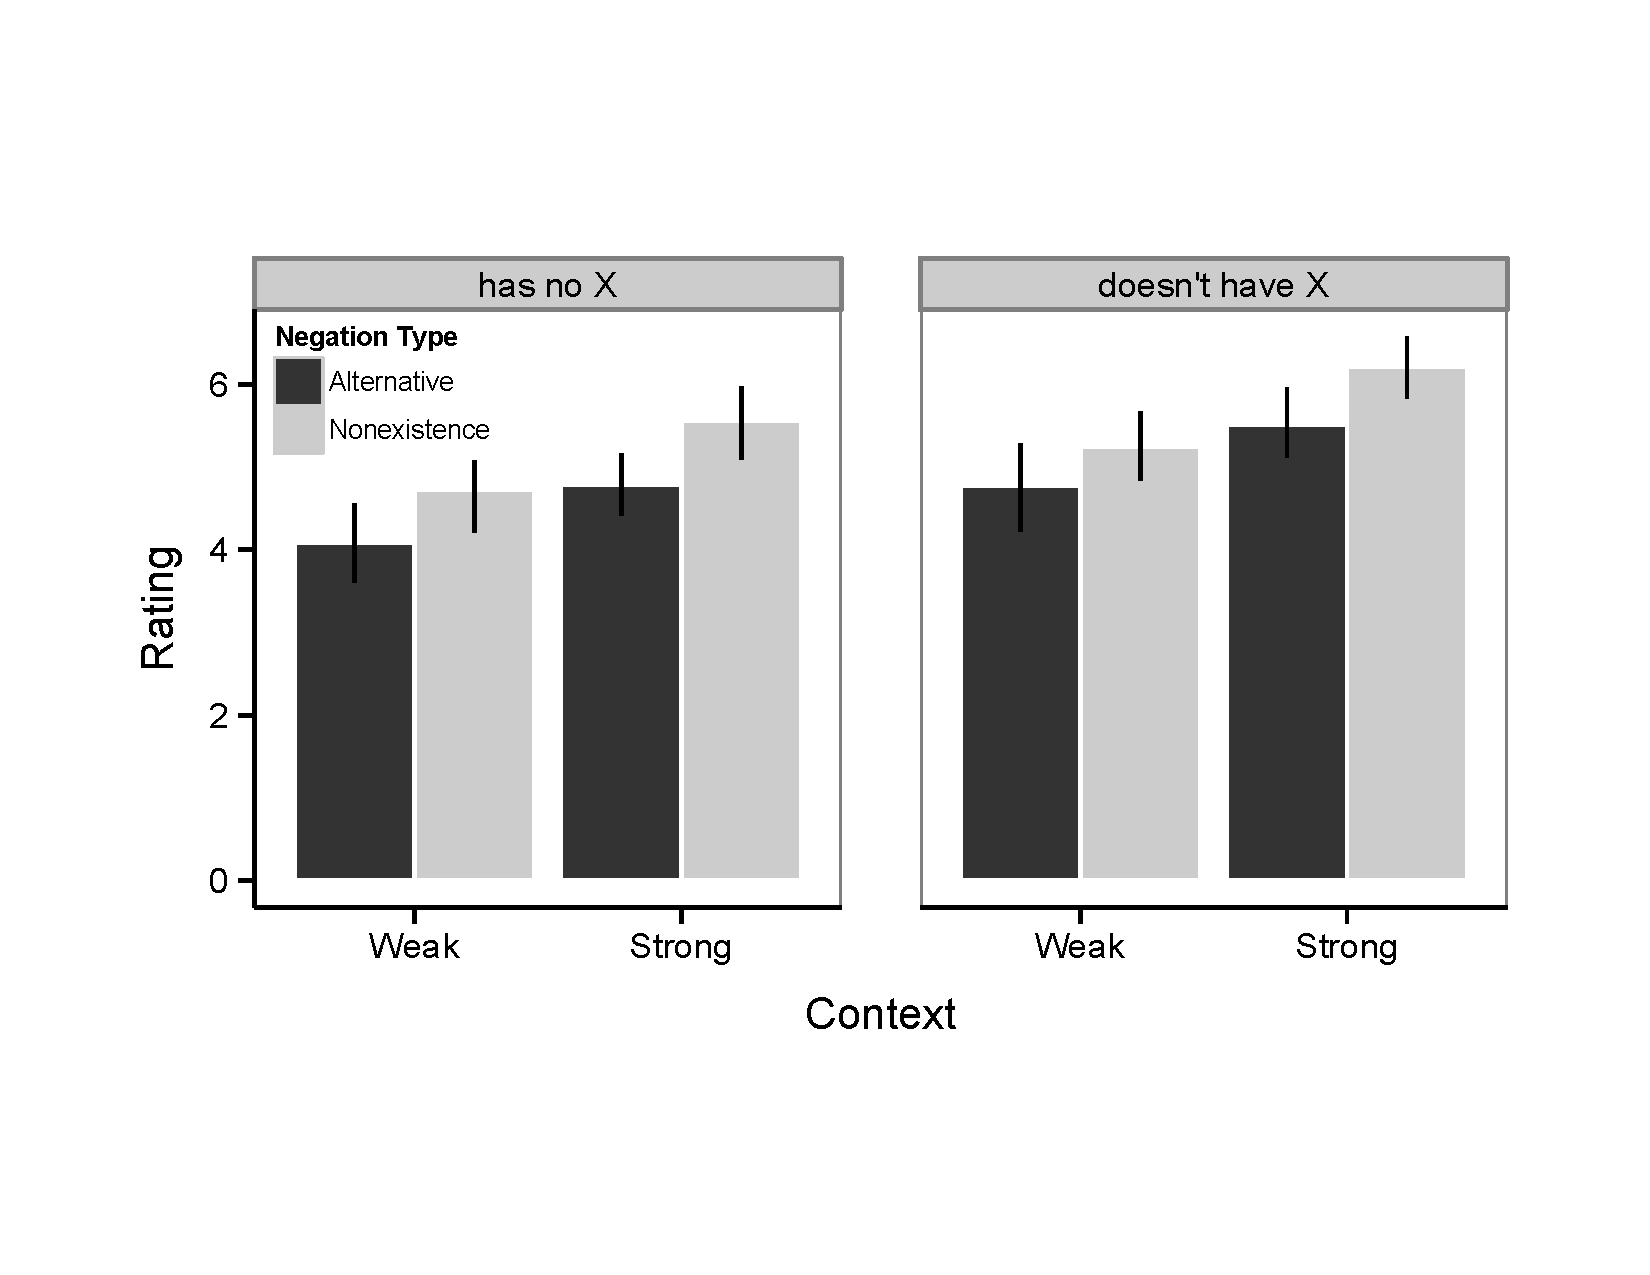
\includegraphics[width=3.25in]{figures/study1.pdf}
\caption{\label{fig:s1} Ratings for different types of true negative sentences in Experiment 1.  Sentences of the form ``...has no X'' are shown on the left, and sentences of the form ``...doesn't have X'' are shown on the right.  Negative sentences expressing nonexistence are shown in black, and negative sentences referring to an alternative object are shown in gray.  Error bars show 95\% confidence intervals.}
\end{center} 
\end{figure}

\begin{table}[t]
\caption{\label{tab:s1} Coefficient estimates from a mixed-effects model predicting true negative sentence ratings in Experiment 1.}
\begin{center}
\small\addtolength{\tabcolsep}{-5pt}
\begin{tabular}{rrrr}
  \hline
 & Coefficient & Std. err. & t value \\ 
  \hline
(Intercept) & 5.28 & 0.19 & 27.16 \\ 
  Context (Context) & 1.08 & 0.27 & 4.04  \\ 
  Negation type (alternative) & -0.43 & 0.17 & -2.50 \\
  Frame (``has no'') & -0.49 & 0.25 & -1.94 \\ 
  Context $\times$Negation type & -0.21 & 0.23 & -.92 \\
  Context $\times$Frame & -0.26 & 0.34 & -0.77 \\
  Negation type$\times$Frame & -0.22 & 0.23 & -0.94 \\
  Context$\times$Negation type$\times$Frame & 0.22 & 0.32 & 0.67 \\
   \hline
\end{tabular}
%\vspace{-1.5cm}
\end{center}
\end{table}

\section{Experiment 2}

In Experiment 2, we examined the effect of three contexts on alternative negation: A \emph{target} context, in which all context characters had the negated target object (identical to Experiment 1), a \emph{none} context, in which none of the context characters had any objects (identical to Experiment 1), and a \emph{foil} context, in which all context characters had an alternative object (e.g. a different object than the one negated in the negative sentences; see Figure \ref{fig:trial}).  Participants saw all three context conditions throughout the experiment, allowing us to examine within-subject effects of context.  

The addition of the ``foil'' context allowed us to test two competing hypotheses about the pragmatics of negation.  In true negative trials with a \emph{foil} context, all characters (including the target character) had the same objects on their table (e.g. cats), and the negative sentence referred to a different object (e.g. ``Abby doesn't have apples'').  Some previous work suggests that a critical element of the effect of context on negative sentences is the fact that the referent of the negative sentence is the ``odd one out'' \cite{wason1965}.  If this is the case, the \emph{foil} context might be even worse than the \emph{none} context, because the target of the negative sentence does not stand out from the context.  If, however, context changes the informativeness of negation, then there should be no difference between the \emph{foil} and \emph{none} contexts, because negative sentences are no less informative in the \emph{foil} context.  

%We also expected to replicate the same difference between the \emph{none} context and the \emph{target} context as was seen in Experiment 1: Negative sentences presented in a \emph{target} context should receive higher ratings than negative sentences presented in a \emph{none} context.  

\subsection{Method}

\subsubsection{Participants}

We recruited 194 participants (115 male, 76 female, three declined to report gender) to participate in an online experiment through Amazon Mechanical Turk.  Participants ranged in age from 18-65.  We restricted participation to individuals in the United States. We paid 40 cents and the experiment took approximately seven minutes to complete.  

\subsubsection{Stimuli}

Trials in Experiment 2 had the same structure as trials in Experiment 1, with a small set of exceptions. First, there were 24 trials. Second, all negative sentences were of the form ``[character] doesn't have a/an [object].'' Third, on each trial, the target character either had a target item on their table, or had an alternative item (eliminating the nonexistence trials).  Each participant evaluated nine true positive sentences, three false positive, three false negative, and nine true negative trials.

In Experiment 2, context was a within-subjects factor with three levels. In the \emph{none} context, context characters had nothing on their table, identical to the \emph{none} context condition in Experiment 1. In the \emph{target} context, context characters each had a target item on their table, same as the \emph{target} context condition in Experiment 1. In the \emph{foil} context, context characters had an alternative item on their table (e.g., all characters have a cat, but the sentence is about the presence/absence of apples; see Figure \ref{fig:trial}).  Each context condition appeared an equal number of times within each trial type.  

\subsubsection{Procedure}

The procedure was identical to Experiment 1.

\subsubsection{Data Processing}

We excluded from our analysis four participants who did not list English as their native language and six participants for having participated in a previous version of the study.  Thus, we analyzed data from a total of 184 participants.  

\subsection{Results and Discussion}

True negative sentences were rated significantly higher when they were presented in a \emph{target} context compared to either the \emph{none} context or the \emph{foil} context (Figure \ref{fig:s2}).  There was no difference between sentences presented in a \emph{foil} context and sentences presented in a \emph{none} context.  As in Experiment 1, context did not affect ratings for true positive sentences or false sentences.  

\begin{figure}
\begin{center} 
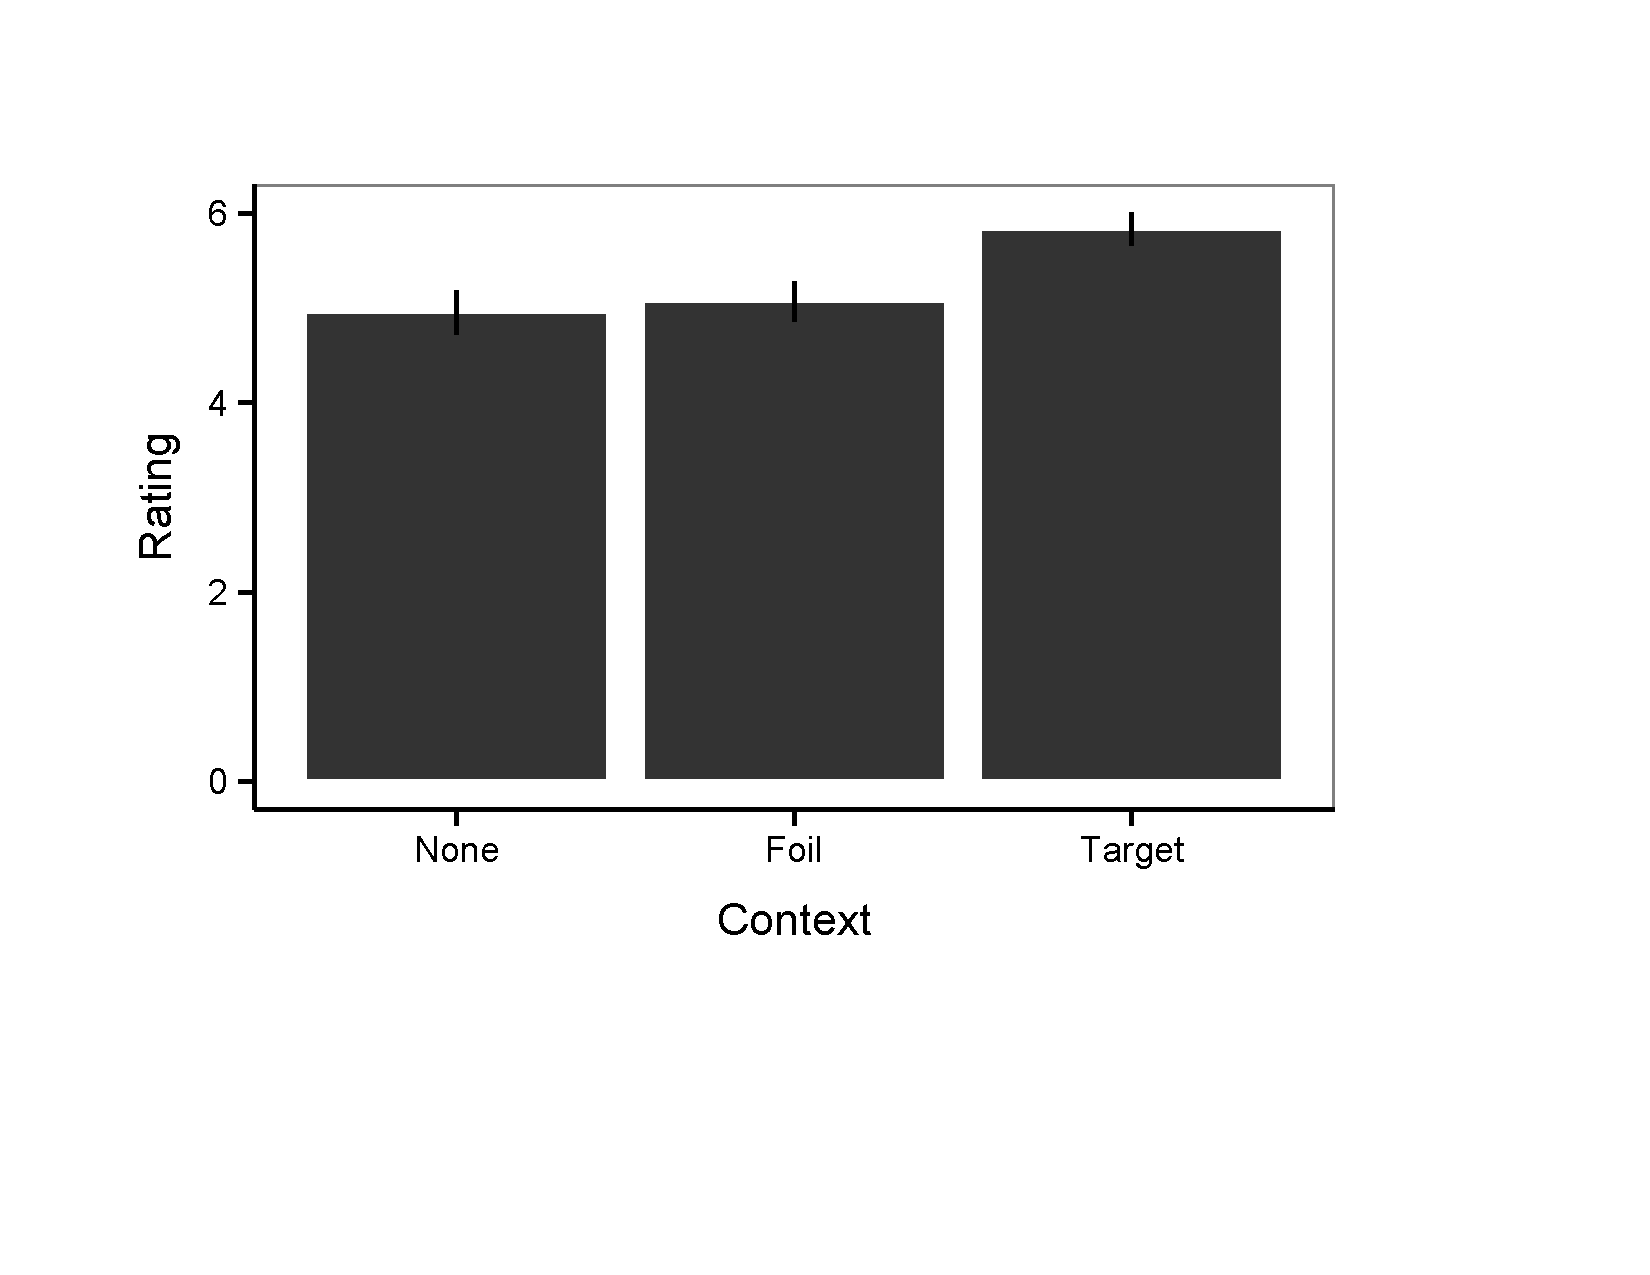
\includegraphics[width=1.8in]{figures/study2.pdf}
\caption{\label{fig:s2} Ratings for true negative sentences in three context conditions in Experiment 2.  Error bars show 95\% confidence intervals.}
\end{center} 
\end{figure}

We fit a linear mixed-effects model to true negative sentence ratings to test the effects of context.\footnote{ The model specification was as follows: \texttt{rating $\sim$ context + (1~\textbar~subject) +  (1~\textbar~item)}}  True negative sentences presented in a \emph{target} context received significantly higher ratings than true negative sentences presented in a \emph{none} context ($\beta= .70$, $p< .001$).  There was no significant difference between sentences presented in a \emph{foil} context and sentences presented in a \emph{none} context ($\beta= .09$, $p=.22$).

In Experiment 2, negative sentences were rated as most felicitous in a context where all of the context characters possessed the negated object.  Negative sentences presented in a \emph{foil} context did not differ significantly from negative sentences in a \emph{none} context.  In the foil context, all characters (including the target character) had the same alternative object.  If the pragmatics of negation require the referent of a negative sentence to be the ``odd one out'' (e.g. lacking a feature that everyone else has), we would expect sentences presented in a \emph{foil} context to be rated lower than sentences presented in the \emph{none} context.  The fact that there was no difference between these two contexts suggests that this is not a necessary feature of a supportive pragmatic context for negation.   Instead, negation appears to be pragmatically licensed in contexts where the negative sentence is highly informative.  

\section{Model}

Both of the preceding studies found a significant effect of context on participants' ratings of true negative sentences.  Why does context have this effect on negative sentences?  One hypothesis is that felicity ratings are influenced by the \emph{informativeness} of negative sentences. On theories of pragmatics, speakers should produce sentences that are appropriately informative based on the context.  In a context where most characters have apples and one does not, it is informative to mention the latter character's lack of apples, because this feature is unique to the character being described.

We used a recent probabilistic model of pragmatics to make predictions about participants' felicity ratings, testing this hypothesis. Details of this model---the ``rational speech act'' model of pragmatics---can be found in a number of previous publications \cite{frank2012,goodman2013,nordmeyer2014}. Here we give a brief sketch of the intuitions behind the model. The probability of a speaker making an utterance in context is defined as being  proportional to the informativeness of the word in context minus its cost.  Informativeness in context is calculated as the number of bits of information conveyed by the utterance.  We assume that the utterance has a uniform probability distribution over its extension in context (e.g., ``doesn't have apples'' applies to any character who does not have apples, leading to a uniform probability of picking out each individual character without apples). We defined cost as the number of words in the utterance multiplied by a cost-per-word parameter; in our simulations, we did not differentiate between different negative sentence frames, and treated negative sentences as having one word more than positive sentences.  Probabilities were normalized over a sparse vocabulary of possible positive or negative utterances that could be used to describe the characters.

\begin{figure}[t]
\begin{center} 
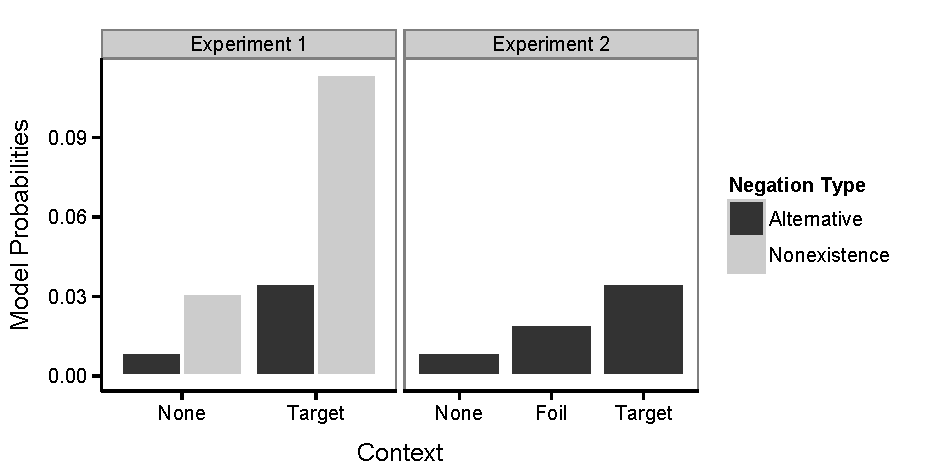
\includegraphics[width=3.25in]{figures/model_predictions.pdf}
\caption{\label{fig:model} Predictions of a model of the informativeness of an utterance in context.  The model predicts how probable a sentence is given a certain context.  Best-fitting parameters were used for this simulation (cost = .8), but the qualitative pattern persists over a wide range of parameter values.  Negative sentences expressing nonexistence are shown in black, and negative sentences referring to an alternative object are shown in gray.}
\end{center} 
\end{figure}

Our model predicted the same qualitative pattern as the data from participants' felicity ratings (Figure \ref{fig:model}).  Sentences presented in a \emph{target} context were preferred over sentences presented in a \emph{none} context, because true negative utterances are more informative when everyone in the context possesses the negated object (e.g., the sentence ``Abby doesn't have apples'' uniquely identifies Abby when every other character \emph{does} have apples).  Nonexistence negation was assigned higher probability than alternative negation, because alternative negation could be described by an equally informative---and less costly---positive utterance (e.g., ``Abby has cats'' instead of ``Abby doesn't have apples'').  Thus, participants' felicity ratings appear to parallel the informativeness of sentences in context.  

\section{General Discussion}

The same negative sentence can sound perfectly fine in one context, but strange in another.  It can refer to \emph{nothing} in one context, but a \emph{difference} in another. In our experiments, we found that contextual differences led to significantly different pragmatic judgments for otherwise identical true grammatical negative sentences.  What is it about the context of negative sentences that elicits these effects?  

The negative sentences that received the lowest felicity ratings across both experiments were alternative negations in a \emph{none} context.  On these trials, participants saw e.g. three characters with nothing, and a character with a cat (see Figure \ref{fig:trial}).  The sentence ``Abby doesn't have apples'' referred to the character with a cat.  Although this sentence is true, it sounds very odd: Why is the speaker talking about Abby's lack of apples, which is true of everyone in the context, instead of mentioning the cat?  Compare this example to nonexistence negation in a \emph{target} context: Three characters have apples, and Abby has nothing.  Here, the same sentence sounds perfectly natural, because Abby's lack of apples is unique, and there is little else to say about her.  In this latter context, producing a negative sentence is reasonable and perhaps even expected.

Previous work on children's acquisition of negation has found that preschoolers struggle to respond correctly to true negative sentences \cite{kim1985, nordmeyer2014b}, despite producing negative sentences spontaneously (and accurately) before they are two years old \cite{pea1980, pea1982}.  One possibility is that children are behaving rationally according to a Gricean view of communication.  In most experiments of children's comprehension of negation, children hear negative sentences without any supportive pragmatic context.  In contrast, studies that have elicited spontaneous negations from children tend to use familiar contexts, such as reading picture books in an interactive, game-like setting \cite{pea1982, hummer1993}.  When children hear a true negative sentence and indicate that it is ``wrong'' \cite<e.g.>{kim1985}, they may be reacting to the infelicity of the sentence rather than its truth value.  

According to Grice's Cooperative Principle, speakers should produce utterances that are maximally informative in order to effectively communicate their intentions to a listener.  If listeners expect speakers to abide by this principle, they should prefer sentences that are more informative.  Our results support this view of communication.  Under a model in which the goal of communication is to convey your intended meaning in the most efficient and effective way possible, negative sentences that were more informative (and therefore more likely to be produced by a speaker) were given higher felicity ratings.  These data suggest that general pragmatic factors, rather than some specific quirk of negation, can explain the relative felicity of different negative sentences in context.  

\section{Acknowledgments}

The first author gratefully acknowledges the support of a National Science Foundation Graduate Research Fellowship. 

\bibliographystyle{apacite}

\setlength{\bibleftmargin}{.125in}
\setlength{\bibindent}{-\bibleftmargin}

\bibliography{negation}


\end{document}
